\documentclass[]{beamer}
\mode<presentation>
{
  \usetheme{Warsaw}
  \definecolor{pstccblue}{rgb}{0, 0.29, 0.56}
  \definecolor{pstccgray}{rgb}{0.6, 0.6, 0.6}
  \setbeamercolor{structure}{fg=pstccblue,bg=pstccgray}
  %\setbeamercovered{transparent}
}


\usepackage[english]{babel}
\usepackage[latin1]{inputenc}
\usepackage{times}
\usepackage[T1]{fontenc}
\usepackage{tikz}
\usepackage{graphicx}
\usepackage{fancyvrb}
\usepackage{adjustbox}

\newcommand{\imagesource}[1]{{\centering\hfill\break\hbox{\scriptsize Image Source:\thinspace{\small\itshape #1}}\par}}

\title{Program Structure}


\author{Dr. Robert Lowe\\}

\institute[Pellissippi State Community College] % (optional, but mostly needed)
{
  Department of Computer Information Technology
  Pellissippi State Community College
}

\date[]{}
\subject{}

\pgfdeclareimage[height=0.5cm]{university-logo}{images/pellissippilogo}
\logo{\pgfuseimage{university-logo}}



\AtBeginSection[]
{
  \begin{frame}<beamer>{Outline}
    \tableofcontents[currentsection]
  \end{frame}
}


\begin{document}

\begin{frame}
  \titlepage
\end{frame}

\begin{frame}{Outline}
  \tableofcontents
\end{frame}


% Structuring a talk is a difficult task and the following structure
% may not be suitable. Here are some rules that apply for this
% solution: 

% - Exactly two or three sections (other than the summary).
% - At *most* three subsections per section.
% - Talk about 30s to 2min per frame. So there should be between about
%   15 and 30 frames, all told.

% - A conference audience is likely to know very little of what you
%   are going to talk about. So *simplify*!
% - In a 20min talk, getting the main ideas across is hard
%   enough. Leave out details, even if it means being less precise than
%   you think necessary.
% - If you omit details that are vital to the proof/implementation,
%   just say so once. Everybody will be happy with that.
\section{Program Structure}

\begin{frame}{Modular Design}
    \begin{itemize}[<+->]
        \item We want to subdivide programs into manageable chunks.
        \item Functions and Structures provide for top-down
            decompositions.
        \item We can decompose further by grouping related functions
            into modules.
        \item In C++, there are no linguistic modules though we tend
            to follow the pattern of 1 module per file.
    \end{itemize}
\end{frame}

\begin{frame}{Multifile Programming}
\begin{columns}
    \column{0.5\textwidth}
    \begin{itemize}[<+->]
        \item Programs typically have multiple source files.
        \item Functions are implemented in \texttt{.cpp} or
        implementation files.
        \item Data types and prototypes are placed in \texttt{.h} or
        header files.
    \end{itemize}

    \column{0.5\textwidth}
    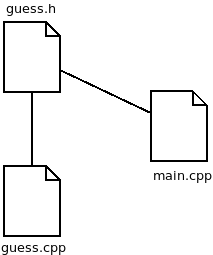
\includegraphics[width=\textwidth]{images/multifile-program}
\end{columns}
\end{frame}

\begin{frame}[fragile]{Header Files}
\begin{columns}
    \column{0.4\textwidth}
    \begin{itemize}[<+->]
        \item Type Definitions
        \item Function Prototypes
        \item Every \texttt{.h} file typically has a corresponding
        \texttt{.cpp} file.
    \end{itemize}

    \column{0.6\textwidth}
    \begin{adjustbox}{max width=\textwidth, max totalheight=0.9\textheight}
    \begin{BVerbatim}
//File: guess.h
//Purpose: Header file for the guessing game module

// Type Definitions

// Function Prototypes
    \end{BVerbatim}
    \end{adjustbox}
\end{columns}
\end{frame}

\begin{frame}[fragile]{Conditional Compilation}
\begin{columns}
    \column{0.4\textwidth}
    \begin{itemize}[<+->]
        \item Prototypes can be repeated.
        \item Type definitions can only appear once in a program.
        \item We use preprocessor directives to protect against
            multiple inclusions.
    \end{itemize}

    \column{0.6\textwidth}
    \begin{adjustbox}{max width=\textwidth, max totalheight=0.9\textheight}
    \begin{BVerbatim}
//File: guess.h
//Purpose: Header file for the guessing game module
#ifndef GUESS_H
#define GUESS_H

// Type Definitions

// Function Prototypes
#endif
    \end{BVerbatim}
    \end{adjustbox}
\end{columns}
\end{frame}

\begin{frame}[fragile]{Implementation File}
\begin{columns}
\column{0.4\textwidth}
\begin{itemize}[<+->]
    \item The implementation files contain lots of C++ functions and
        code.
    \item The main function typically gets its own file, which I like
        to name \texttt{main.cpp}.  
    \item I am a creative fellow, after all.
\end{itemize}

\column{0.6\textwidth}
    \begin{adjustbox}{max width=\textwidth, max totalheight=0.9\textheight}
    \begin{BVerbatim}
//File: guess.cpp
//Purpose: This is the implementation of the guessing game functions.
#include "guess.h"

//C++ Code for Functions Goes Here
    \end{BVerbatim}
    \end{adjustbox}
\end{columns}
\end{frame}

\begin{frame}{Activity: Refactor Guessing Game}
    \begin{enumerate}
        \item Make a directory to store the guessing game.
        \item Copy the \texttt{guess.cpp} example into this directory.
        \item Refactor the program into the following modules:
        \begin{itemize}
            \item \texttt{guess.h, guess.cpp}
            \item \texttt{score.h, score.cpp}
            \item \texttt{main.cpp}
        \end{itemize}
        \item Add the following feature:
            \newline After each game, ask the player if they want to
                play again.  If they do, play again! (new number and all)
    \end{enumerate}
\end{frame}

\begin{frame}[fragile]{Compiling a Program with Multiple Files}
    \begin{BVerbatim}
    g++ guess.cpp score.cpp main.cpp -o guess
    \end{BVerbatim}
\end{frame}

\section{The Build Process}

\begin{frame}{Multi-Stage Compilation}
\begin{itemize}[<+->]
    \item Compiling the entire source every time is quite
    time consuming.
    \item Instead we split the compilation into two parts:
    \begin{enumerate}
        \item Compile \texttt{cpp} files.
        \item Link \texttt{cpp} files together.
    \end{enumerate}
    \item We can do this by adding the \texttt{-c} option to
        \texttt{g++}
\end{itemize}
\end{frame}

\begin{frame}[fragile]{Multi-Stage Compilation of the Guessing Game}
    Try the following sequence of commands:
    \begin{BVerbatim}
        g++ -c main.cpp
        g++ -c guess.cpp
        g++ -c score.cpp
        g++ main.o guess.o score.o -o guess
    \end{BVerbatim}
\end{frame}

\begin{frame}{Enter Make}
\begin{itemize}[<+->]
    \item Linking object files is faster than compiling source files.
    \item We only need to recompile the object files when the source
        file changes.
    \item This is still a heavy workload!
    \item This where the tool \texttt{make} comes in.
    \item \texttt{make} lets us script the build process in an
        intelligent way.
    \item \texttt{make} works by processing ``recipes''.
    \item Recipes are either implicit or explicitly.
\end{itemize}
\end{frame}

\begin{frame}[fragile]{Implicit Recipes}
\begin{itemize}[<+->]
    \item Make is scripted by creating a file named ``\texttt{Makefile}''
    \item In the \texttt{Makefile} we write a series of
        \textbf{recipes} in the following format:
        \newline\texttt{target: ingredient list}
    \item Make is ``smart enough'' to build some things without extra
        input.
    \item For instance, Create a new file called ``\texttt{Makefile}''
    and enter the following:
    \newline\begin{BVerbatim}
main.o: main.cpp guess.h score.h
    \end{BVerbatim}

    \item Now try the following commands:
    \newline\begin{BVerbatim}
    rm main.o
    make
    \end{BVerbatim}
\end{itemize}
\end{frame}


\begin{frame}[fragile]{Makefile -- Explicit Recipes}
\begin{itemize}[<+->]
    \item When we compile multiple files, we need to explicitly tell
        make how to go about doing it.
    \item For example, try the following:
    \begin{enumerate}
        \item Modify your \texttt{Makefile} to read as follows:
\begin{adjustbox}{max width=\textwidth, max totalheight=0.9\textheight}
\begin{BVerbatim}
guess: main.o guess.o score.o
    g++ main.o guess.o score.o -o guess
main.o: main.cpp guess.h score.h
guess.o: guess.cpp guess.h
score.o: score.cpp score.h
\end{BVerbatim}
\end{adjustbox}
    \end{enumerate}
    \item Remember that when indenting, you must use a literal tab
        character!
    \item Try running \texttt{make} now!
\end{itemize}
\end{frame}


\begin{frame}[fragile]{Some Predefined Variables}
\begin{itemize}[<+->]
    \item The make syntax is itself a scripting language.
    \item Variables begin with dollar signs \$.  
    \item There are several pre-defined variables, the two most
        commonly used ones are:
        \begin{itemize}
            \item \verb!$@! -- The name of the target
            \item \verb!$^! -- The list of all ingredients
        \end{itemize}
    \item We could simplify our \texttt{Makefile} like so:
\begin{adjustbox}{max width=\textwidth, max totalheight=0.9\textheight}
\begin{BVerbatim}
guess: main.o guess.o score.o
    g++ $^ -o $@
main.o: main.cpp guess.h score.h
guess.o: guess.cpp guess.h
score.o: score.cpp score.h
\end{BVerbatim}
\end{adjustbox}
\end{itemize}
\end{frame}


\begin{frame}{User Defined Variables}
\begin{itemize}[<+->]
    \item You can also define your own variables:
        \newline \texttt{TARGETS=guess}
    \item You refer to your own variables like this:
        \newline  \texttt{\$(TARGETS)}
    \item This allows you to make compact makefiles.
\end{itemize}
\end{frame}

\begin{frame}[fragile]{Making The Program 5 Makefile}
\begin{adjustbox}{max width=\textwidth, max totalheight=0.9\textheight}
\begin{BVerbatim}
TARGETS=guess

#application builds
all: $(TARGETS)
guess: main.o guess.o score.o
    g++ $^ -o $@

#module builds
main.o: main.cpp guess.h score.h
guess.o: guess.cpp guess.h
score.o: score.cpp score.h

#delete all binaries
clean:
	rm -f *.o $(TARGETS)
\end{BVerbatim}
\end{adjustbox}
\end{frame}

\begin{frame}{Building With Make}
    \begin{itemize}[<+->]
        \item Run \texttt{make} to build the first recipe in the
            \texttt{Makefile}
        \item Run \texttt{make target} to build any other target.
        \item For example \texttt{make clean} runs the clean target.
        \item Each time you run \texttt{make}, it only does the
            minimal number of steps to complete the build!
    \end{itemize}
\end{frame}


\end{document}


